\documentclass{ML}

% 姓名,学号
\infoauthor{朱明彦}{1160300314}

% 课程类型,实验名称
\infoexp{课程类型}{概述}

\infoschool{计算机学院}{高宏}

\begin{document}
\maketitle

\tableofcontents
\newpage

\begin{center}
    \textbf{\zihao{3} 论文概述}
\end{center}

\section{解决的问题}
选择的论文\cite{toain}为2018年PVLDB上面的一篇文章,\textbf{主要解决的问题是Road Networks上面动态的kNN查询}。

针对这个问题,作者主要有如下\textbf{三个方面}的工作:
\begin{enumerate}
    \item 对于Road Networks上需要进行kNN查询的系统建立新的数学模型,并找到其中影响系统整体吞吐量的关键因素。
    \item 建立了一个以Shortcut Graph为基础的索引,SCOB。
    \item 设计了可以调整SCOB以最大化系统吞吐量的算法,TOAIN。
\end{enumerate}
\section{采用的思想}
作者为了解决Road Networks上面动态的kNN查询,采用的思想是\textbf{先明确系统的目标(最大化系统的吞吐量),建立数学模型衡量寻找影响体统吞吐量的关键因素,对于关键的因素建立索引并利用设计的算法尽量提高关键因素影响下的部分,最终实现最大化吞吐量的目的}。

\begin{figure}[htb]
	\centering
	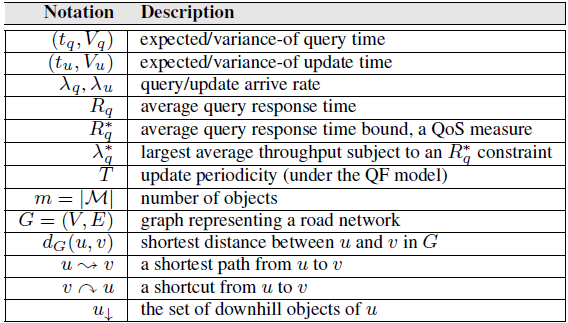
\includegraphics[width=0.8\linewidth]{media/notations.png}
	\caption{Notations}\label{fig:notations}
\end{figure}
\subsection{数学模型方面}
作者主要考虑了两种不同的情况,分别对应于现实中两种不同的应用,即\textbf{如滴滴类似的打车软件系统和捕捉精灵球的Pokemon}。 作者在考虑数学模型时,从\textbf{Query}和\textbf{Update}分别考虑其影响,然后针对这两种不同的应用区分它们在Query和Update上面的差别,从而建立起来不同的数学模型。

\textbf{以下两种应用都假设所有的查询到来是随机的,论文中为了方便假设Query符合泊松过程(Poisson Process)。}
\paragraph{打车软件(BUA+QF Model)}
\textbf{BUA模型是针对Update操作来说},其假设所有的元素都会进行Update操作,且都是在时间片的开始时刻进行,如果在某一个时间片里没有完成相应的Update操作,则直接舍弃未做操作,进行下一轮操作即可。\textbf{QF(Query First)是针对Query\\操作来说},其假设Query的优先级高于Update。

基于上面的假设,在打车软件这样的系统中,对于每个Query是来自用户的,查询在其附近最近的K个车辆;每个Update是来自汽车的,其在指定间隔内向系统返回其最新的位置。这样,高优先级的Query可以尽量减少用户请求的查询的延迟,并且丢失少量Update使得某些车辆的信息具有很短距离的差距,所以这样的假设对于该应用是合理的。

利用在\cite{single-server-queue}中的结论,可以得到式\eqref{equ:1},其中$R_q$为平均查询响应时间,$t_q, V_{q}$分别是查询时间的期望和方差,$\lambda_{q}$为Query到达的速率,即泊松过程中的参数。
\begin{equation}
R_{q}=\frac{\lambda_{q}\left(t_{q}^{2}+V_{q}\right)}{2\left(1-\lambda_{q^{t} q}\right)}+t_{q}
\label{equ:1}
\end{equation}

通过式\eqref{equ:1}可以看到,\textbf{整体的查询响应时间随$\lambda_{q}$的增大而增大,这也与我们的直觉相符合,说明此模型具有一定的道理}。进而通过两个约束,\textbf{查询的响应时间不能超过用户能够忍受的最大值}和\textbf{在一个时间间隔内需要最少的用于Update的时间限制},得到最终的$\lambda_{q}$的上界,如式\eqref{eq:2}所示。

\begin{equation}
\lambda_{q}^{*} \leq \min \left\{\frac{2\left(R_{q}^{*}-t_{q}\right)}{V_{q}+2 R_{q}^{*} t_{q}-t_{q}^{2}}, \quad\left(T-m t_{u}\right) /\left(T \cdot t_{q}\right)\right\}
\label{eq:2}
\end{equation}

为了可解释性,将式\eqref{eq:2}转化为式\eqref{eq:3}。
\begin{equation}
\lambda_{q}^{*} \leq \left\{
\begin{array}{lll}
{1 / t_{q},} & {\text { if } \alpha \beta<1 / 2} & {(\text { QoS-bound mode })} \\ 
{(1-\beta) / t_{q},} & {\text { if } \alpha \beta \geq 1 / 2} &\text {(Update-bound mode)}
\end{array}
\right.
\label{eq:3}
\end{equation}

其中$\alpha=R_{q}^{*} / t_{q} ; \quad \beta=m t_{u} / T ; \quad \gamma=V_{q} / t_{q}^{2}$;$\alpha$用来衡量平均查询相应时间的上界与平均查询时间的比值,$\beta$用来衡量一个时间片内处理Update所用时间的占比,$\gamma$是离散系数(coefficient of variation)的平方,相对于标准差其为无量纲量可以用在不同的索引算法中进行比较,一般$\gamma \in [0.1, 0.9]$。	

\paragraph{Pokemon游戏(RUA+FCFS模型)}
% TODO
\subsection{索引SCOB方面}
\subsection{算法TOAIN方面}
\section{基本算法描述}
文中以伪代码形式讲述的算法共有4个,下面将分别进行描述。
\subsubsection{SCOB Index}
\paragraph{Query}
\begin{figure}[htb]
	\centering
	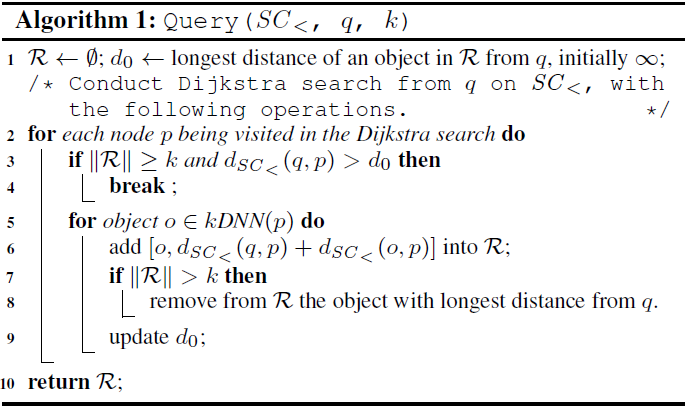
\includegraphics[width=0.8\linewidth]{media/query.png}
	\caption{Query Algorithm}\label{fig:query}
\end{figure}
\paragraph{Insert}
\begin{figure}[htb]
	\centering
	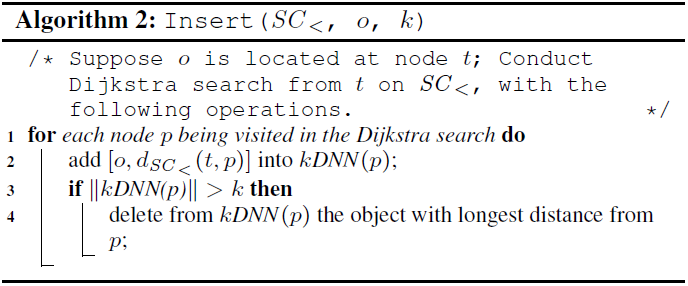
\includegraphics[width=0.8\linewidth]{media/insert.png}
	\caption{Insert Algorithm}\label{fig:insert}
\end{figure}
\paragraph{Delete}
\begin{figure}[htb]
	\centering
	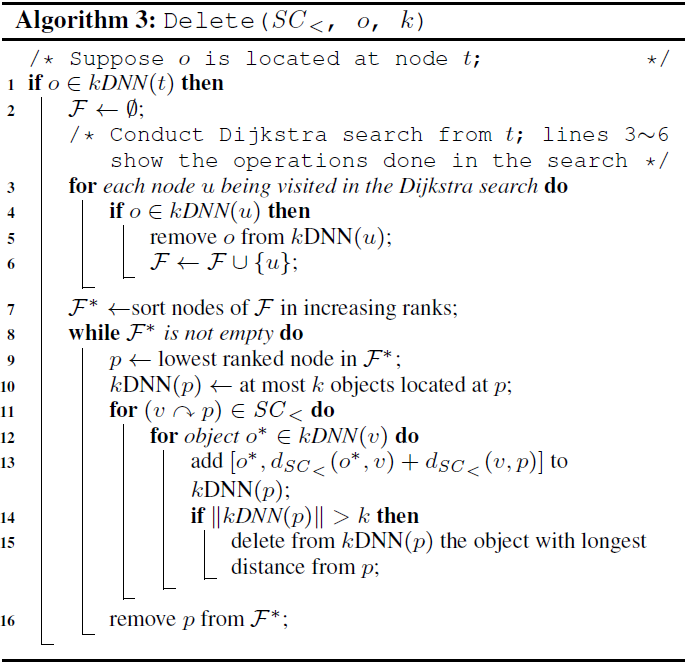
\includegraphics[width=0.8\linewidth]{media/delete.png}
	\caption{Delete Algorithm}\label{fig:delete}
\end{figure}
\subsubsection{TOAIN}
\paragraph{Compute Rank}
\begin{figure}[htb]
	\centering
	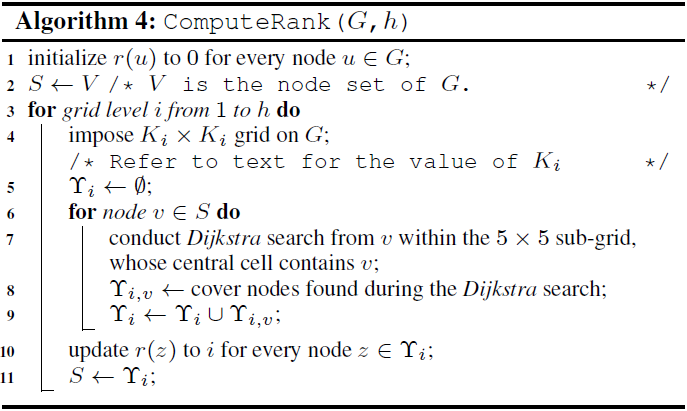
\includegraphics[width=0.8\linewidth]{media/compute_rank.png}
	\caption{Compute Rank Algorithm}\label{fig:compute_rank}
\end{figure}
\section{算法分析}

\section{举例说明}

\appendix

% \section{源代码}
% \section{参考文献}
\begin{thebibliography}{20}
    \bibitem{toain} Luo, S., Kao, B., Li, G., Hu, J., Cheng, R., \& Zheng, Y. (2018). TOAIN: a throughput optimizing adaptive index for answering dynamic k NN queries on road networks. Proceedings of the VLDB Endowment, 11(5), 594-606.
    \bibitem{single-server-queue} J. W. Cohen. The single server queue, volume 8. Elsevier, 2012.
\end{thebibliography}

\end{document}
